\subsection{Election November 5, 1912: *Wilson vs Roosevelt}
\begin{frame}[t]{Election November 5, 1912: *Woodrow Wilson}
\small
% Wilson
\begin{columns}[T, onlytextwidth]
\column{0.48\textwidth}
\vspace{-1em}
{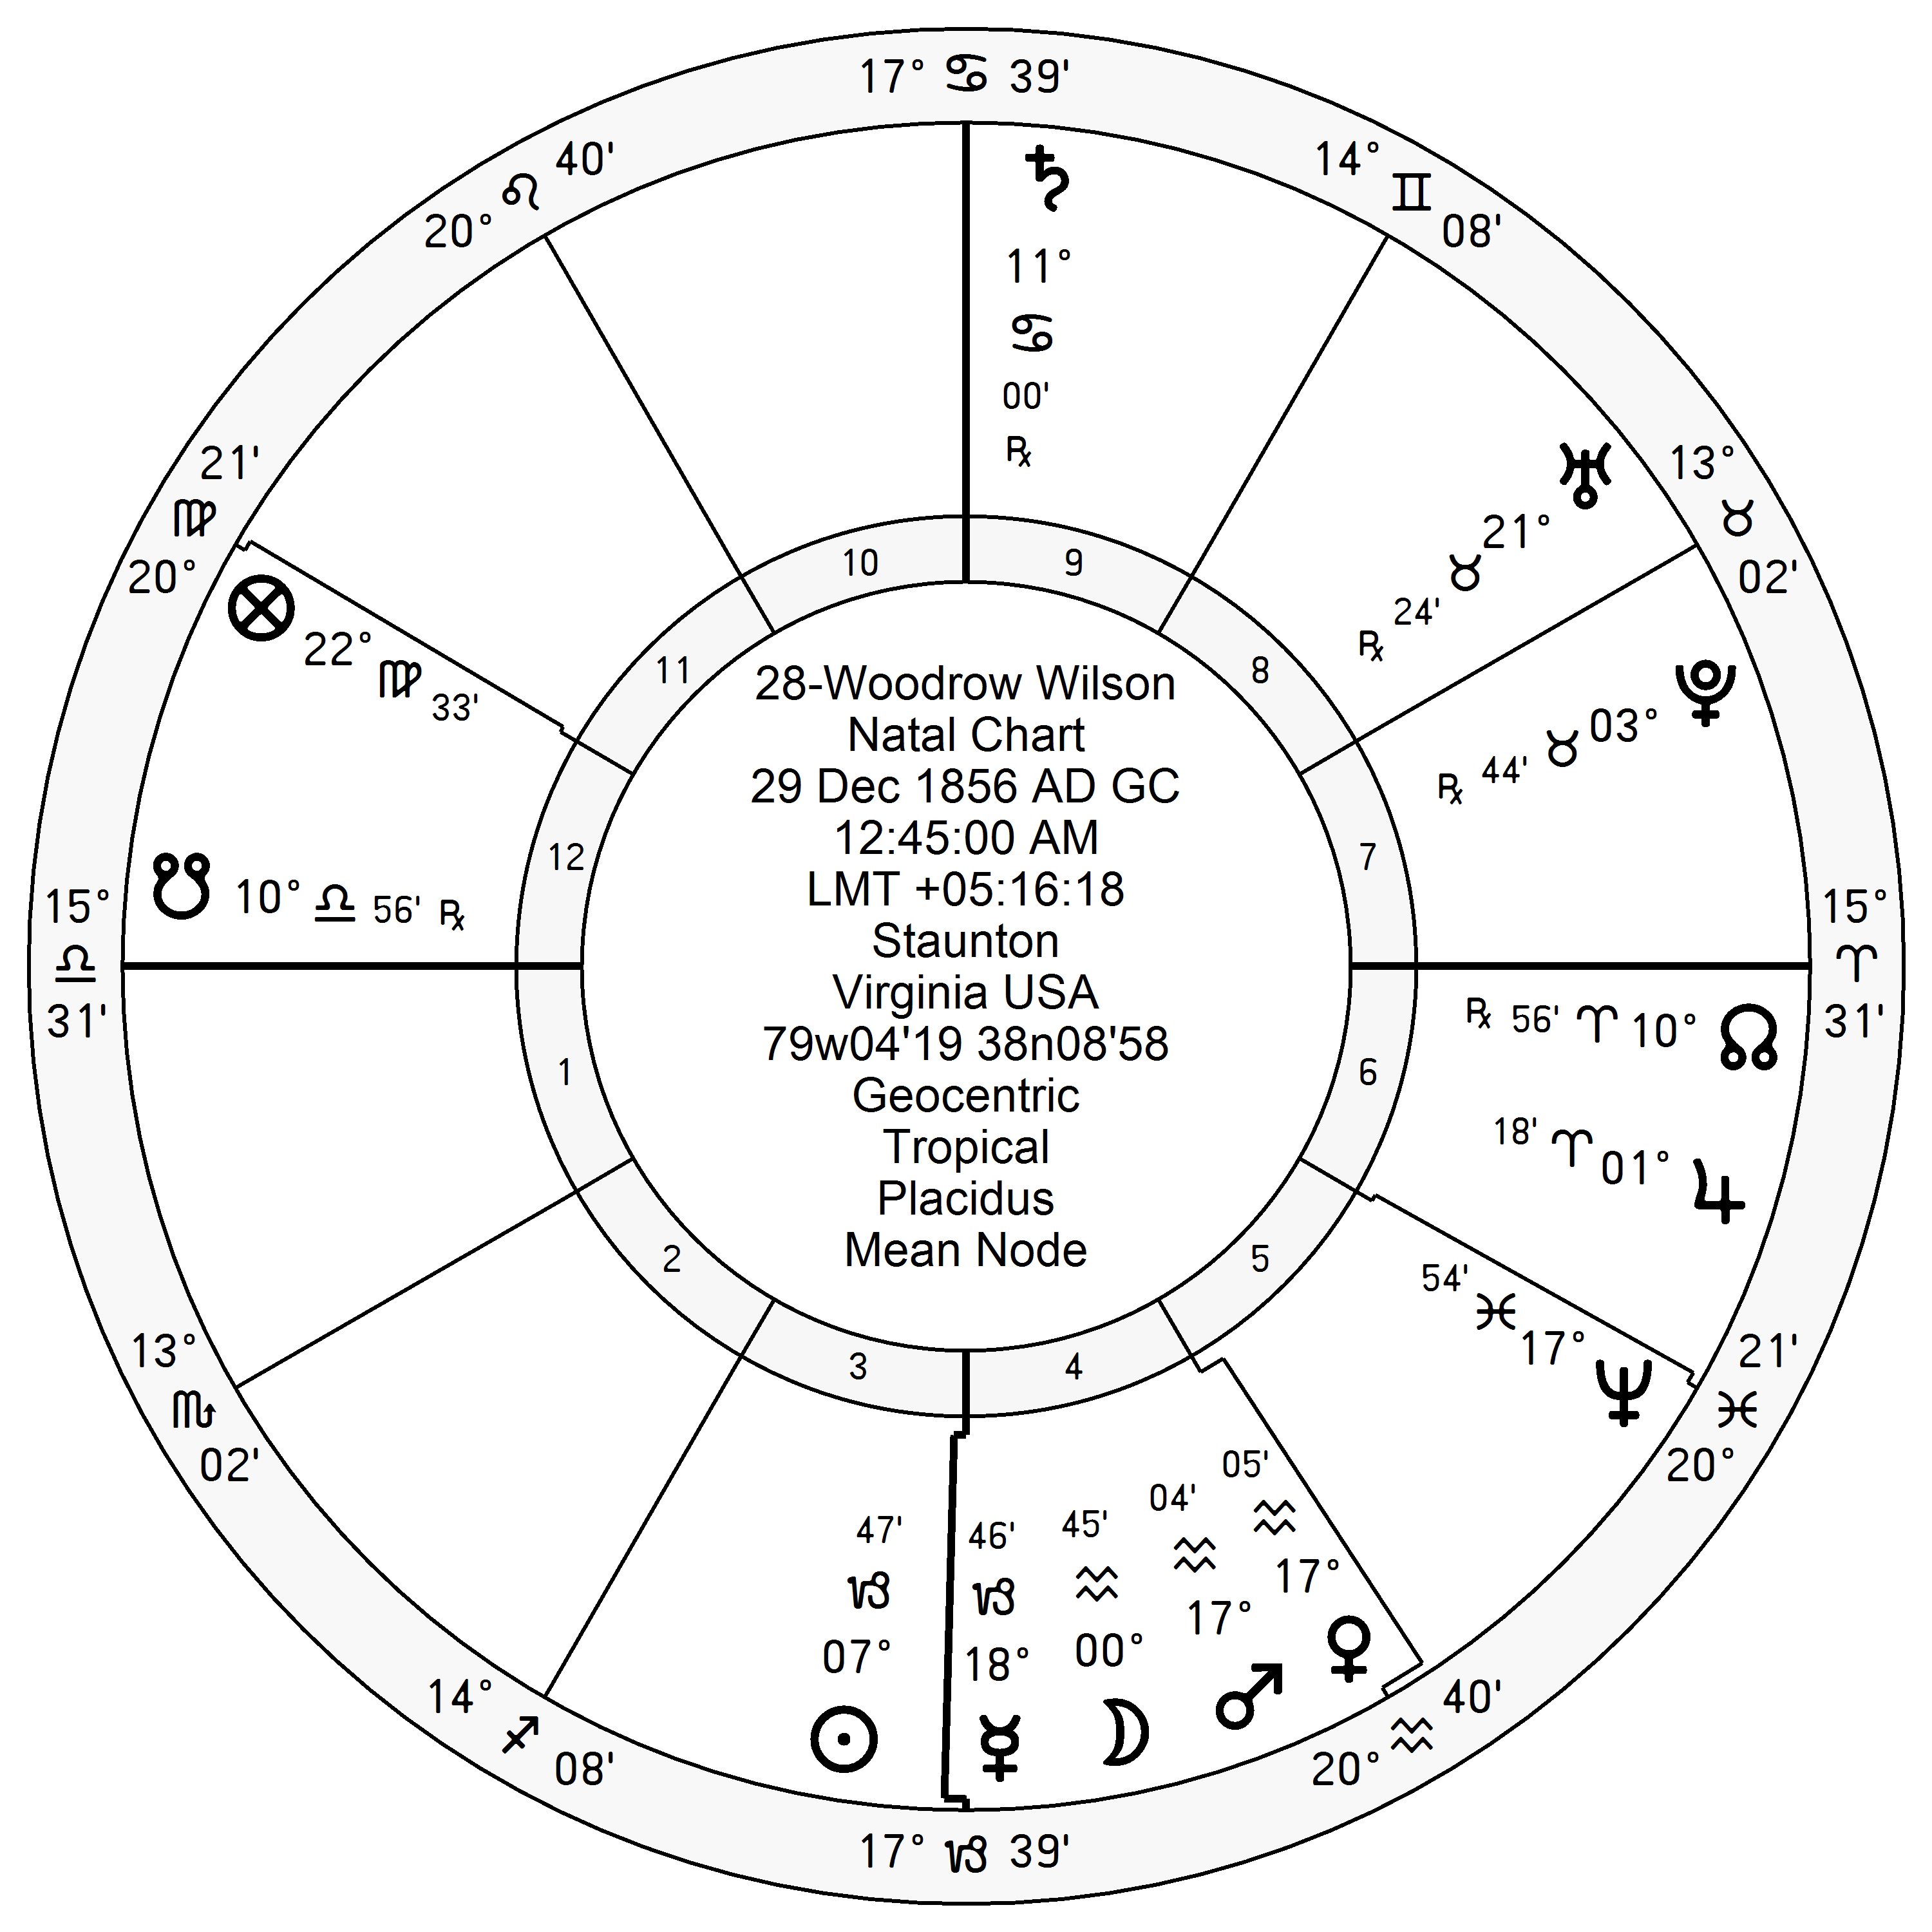
\includegraphics[width=0.9\textwidth]{charts/Wilson.png}}
\fontsize{7pt}{8pt}\selectfont

\Venus\, in P10, \Opposition\, N10; \Square\, P1, \Trine\, N1 \\
\Saturn\, \Trine\, P10 \\
\Jupiter\, makes no aspects to P1, N1 or P10, N10

\column{0.48\textwidth}
\vspace{-1em}
{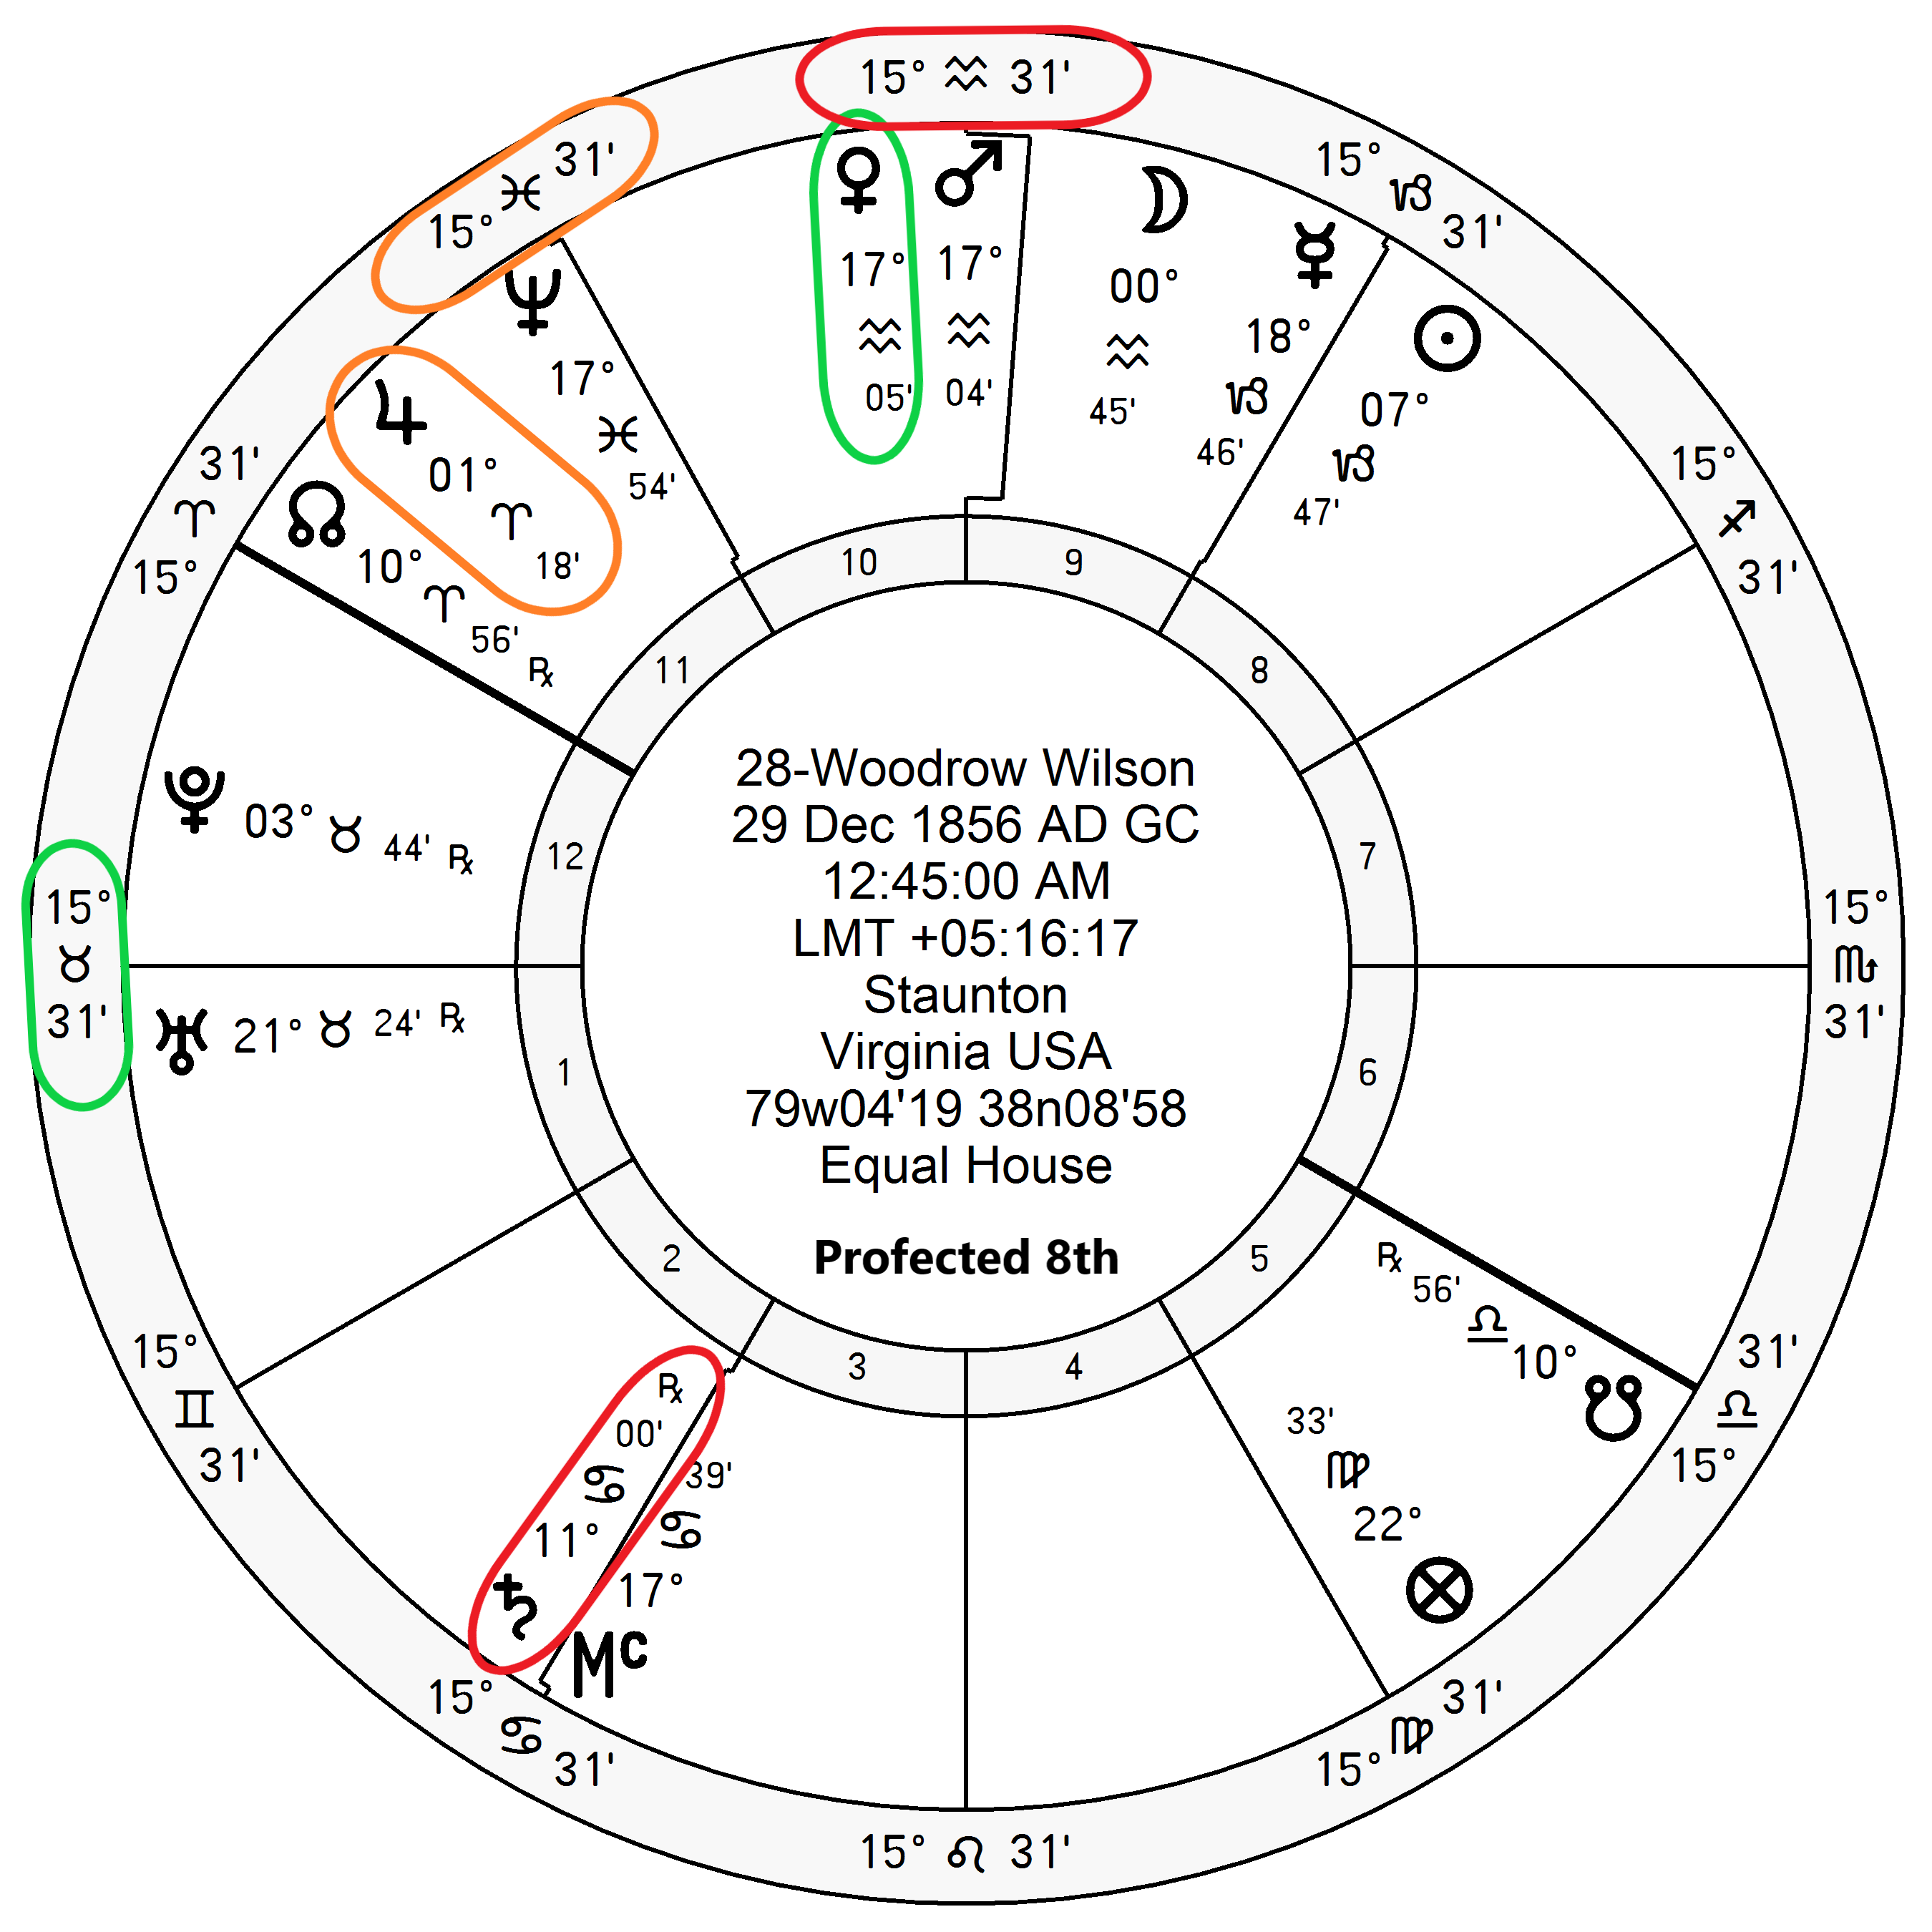
\includegraphics[width=0.9\textwidth]{charts/Wilson-Prof-8th.png}}

\textbf{\dgreen P1}=N8
	$\Rightarrow$ \Venus\, $\Rightarrow$ \textbf{\red P10}/N4 \\
\textbf{\red P10}=N5
	$\Rightarrow$  \Saturn\,\Retrograde $\Rightarrow$ P2/N9 \\
PE=P11/N6
	$\Rightarrow$  \Jupiter\, $\Rightarrow$  P11/N6

\end{columns}
\end{frame}

% Roosevelt
\begin{frame}[t]{Election November 5, 1912: Teddy Roosevelt}
\small
\begin{columns}[T, onlytextwidth]
\column{0.48\textwidth}
\vspace{-1em}
{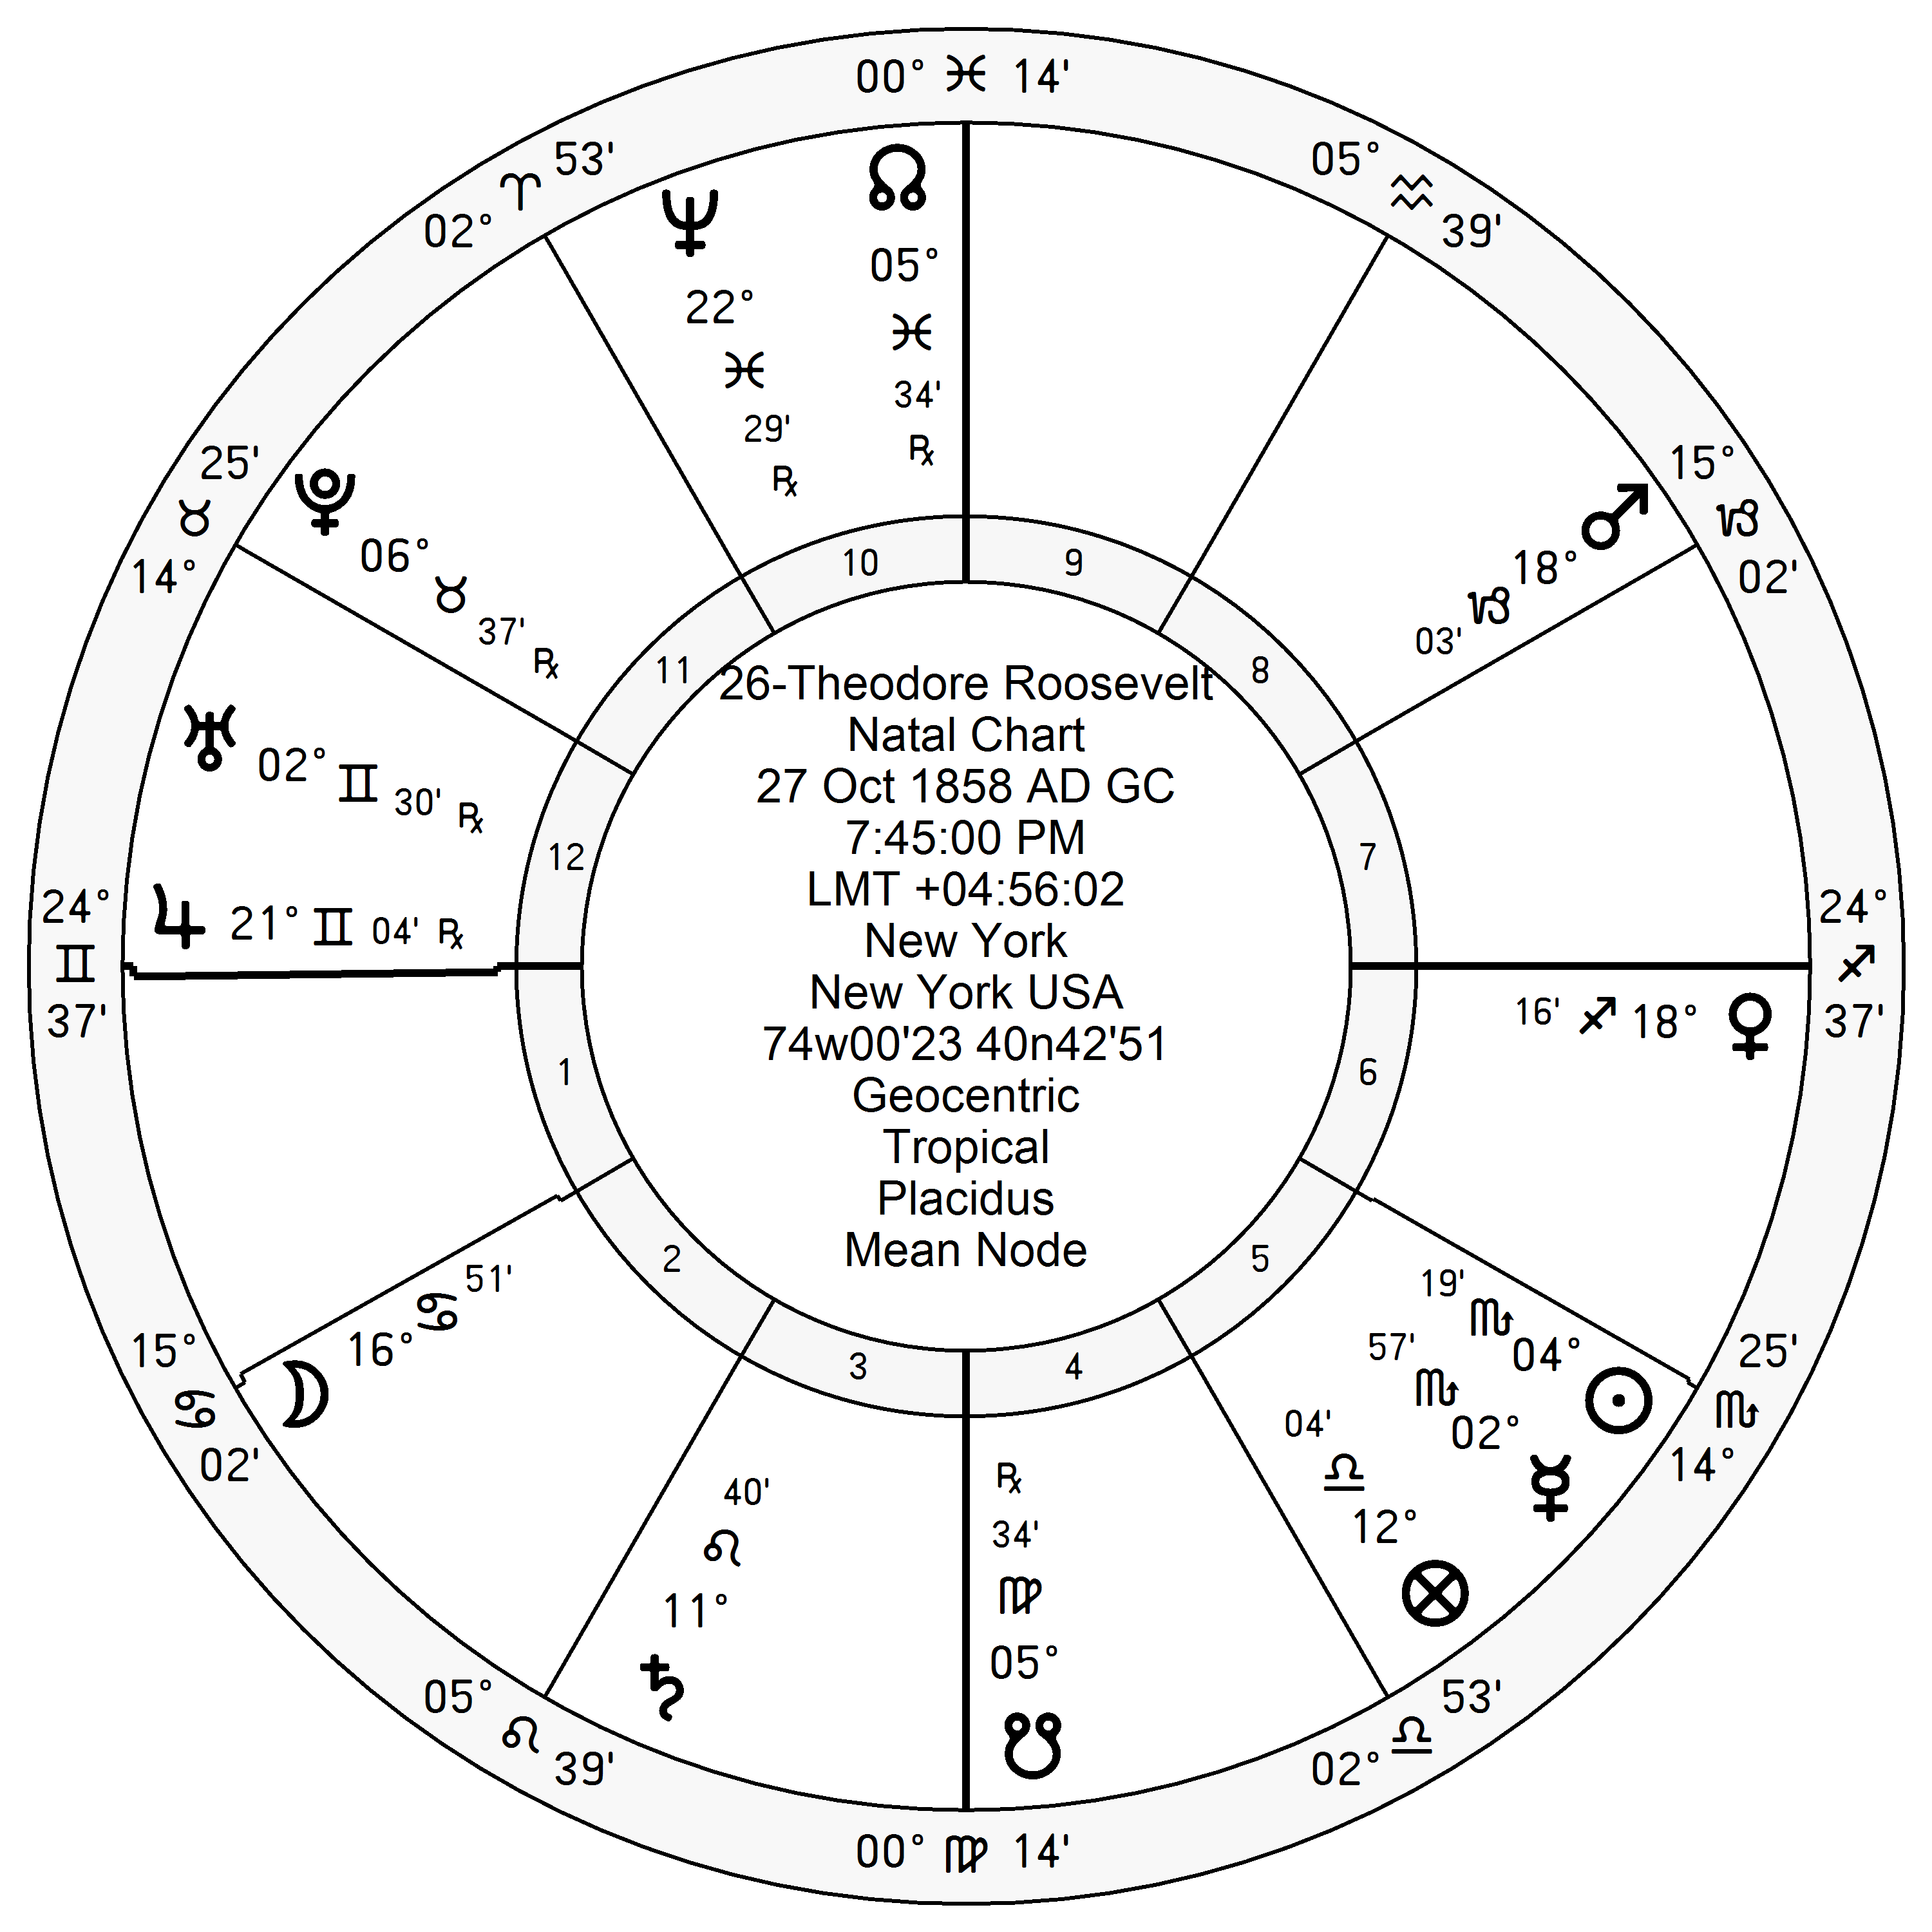
\includegraphics[width=0.9\textwidth]{charts/Roosevelt.png}}
\fontsize{8pt}{9pt}\selectfont

\Jupiter\, \Square\, N10 (1° from \Neptune) \\
\Mercury\, combust; \Trine\, N10

\column{0.48\textwidth}
\vspace{-1em}
{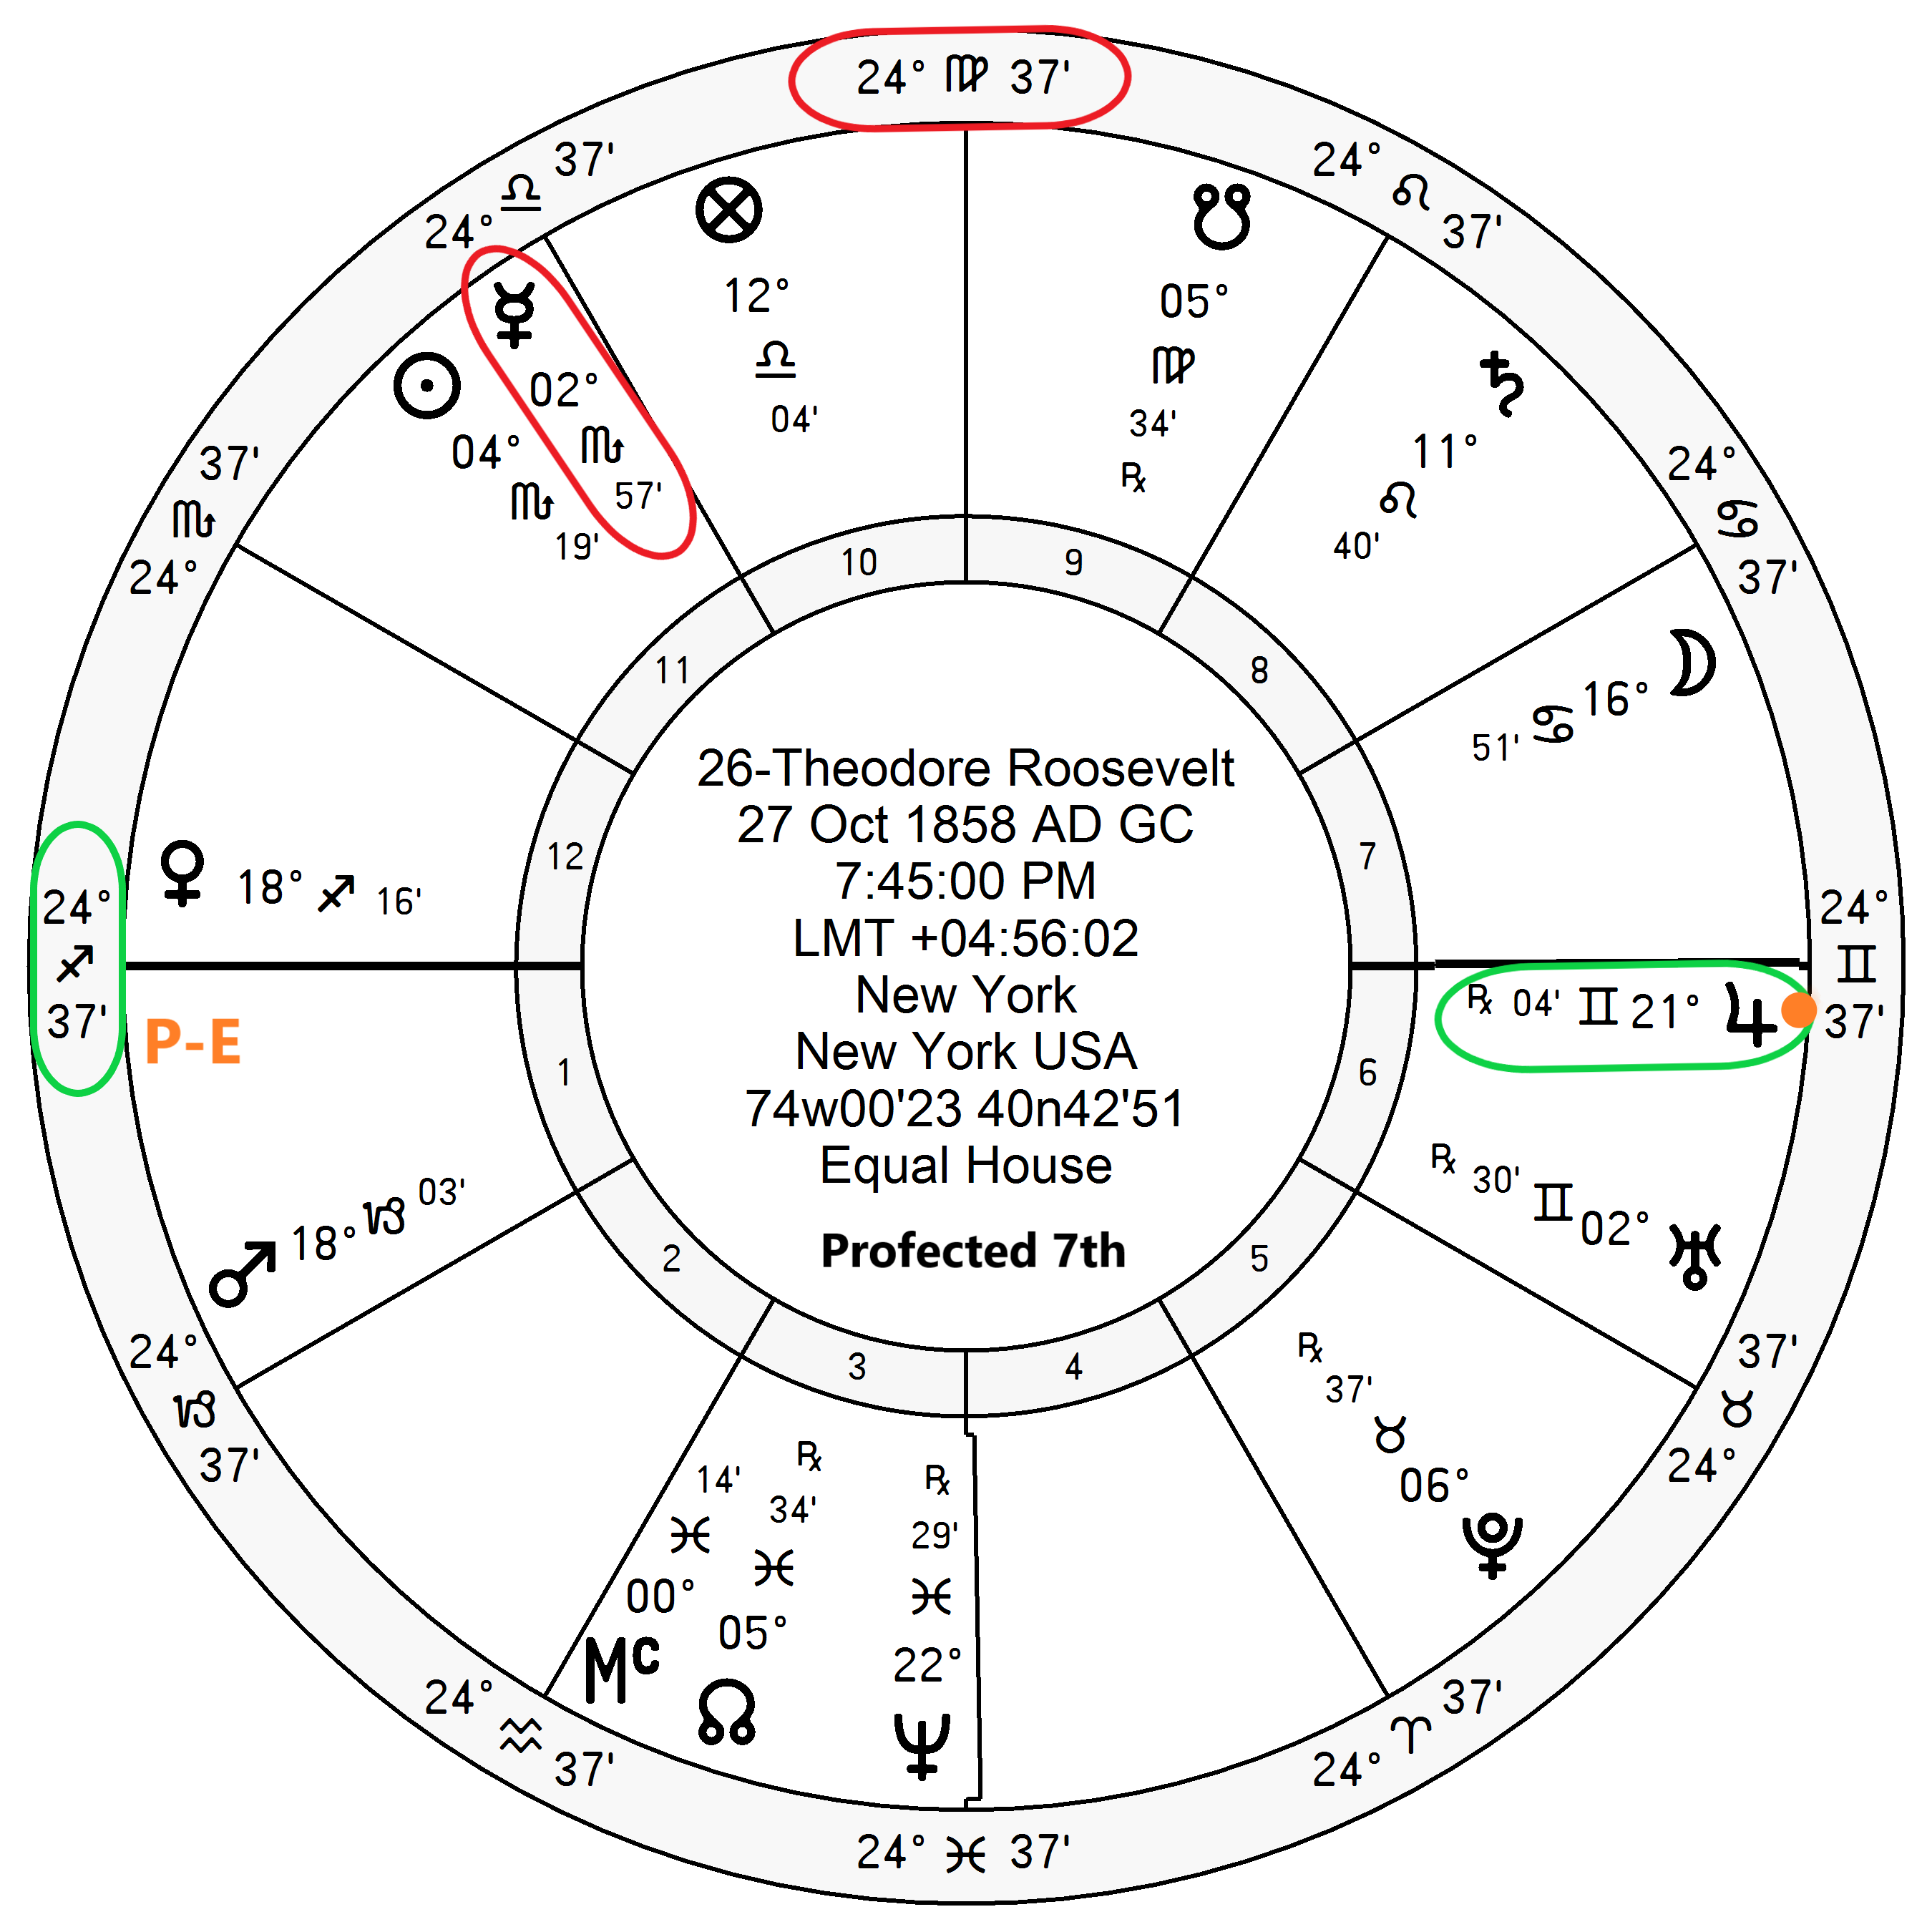
\includegraphics[width=0.9\textwidth]{charts/Roosevelt-Prof-7th.png}}
\textbf{\dgreen P1=N7} 
	$\Rightarrow$ \Jupiter\,\Retrograde $\Rightarrow$ \textbf{\dgreen P6/N12}\\
\textbf{\red P10}=N4
	$\Rightarrow$ \Mercury\, (combust) $\Rightarrow$ P11/N5\\
PE=\textbf{\dgreen P1/N7}
	$\Rightarrow$ \Jupiter\,\Retrograde $\Rightarrow$ \textbf{\dgreen P6/N12}


\end{columns}
\end{frame}
